\documentclass{article}
\usepackage[dblblindworkshop,final]{neurips_2026}
\workshoptitle{Linguistic Principles for Foundation Models (LP4FM)}

\usepackage[utf8]{inputenc}
\usepackage[T1]{fontenc}
\usepackage{amsmath,amssymb}
\usepackage{booktabs}
\usepackage{array}
\usepackage{microtype}
\usepackage[hidelinks]{hyperref}
\usepackage{xcolor}
\usepackage{graphicx}

\usepackage{listings}
\lstset{
  language=Python,
  basicstyle=\ttfamily\footnotesize,
  breaklines=true,
  breakatwhitespace=true,
  columns=fullflexible,
  keepspaces=true,
  showstringspaces=false,
  xleftmargin=1em,
  literate={—}{{\textemdash}}1 {“}{{\textquotedblleft}}1 {”}{{\textquotedblright}}1 {‘}{{\textquoteleft}}1 {’}{{\textquoteright}}1,
}

\title{Burstiness Was Measured Wrong, and Prompting Cannot Aim It}

\author{Anonymous Author(s)\\
  Affiliation\\
  Address\\
  \texttt{email}}

\begin{document}
\maketitle

\begin{abstract}
\noindent
Burstiness is a signal people already use to judge machine text, and its
operational definition in practice is an unreviewed detector heuristic
confounded with length: raw sentence-length variance grows with the mean.
We treat sentence boundaries as a point process in word-time, scored with
the Goh--Barab\'asi coefficient under the Kim--Jo finite-$n$ correction:
bounded and scale-free, no model in the loop, screened by a Goodhart guard
and a coherence gate. The protocol is paired evaluation on $200$ era-,
topic-, and register-matched Wikinews articles dated 2016--2021: five prompting
modes, nine model families, three seeds, uniform normalization of generated
text before scoring. Scored raw, markdown scaffolding manufactures
dispersion and produces a parity verdict that normalization reverses
(instruction-mode $0.005$, $p=0.10$, becomes a significant $0.028$ deficit,
$p=3\times10^{-5}$), and the uninstructed dispersion gap more than doubles
($0.043$ to $0.097$). Of the forty-five family-by-mode cells, thirty-two
land significantly flatter than the human articles, eight show no significant
difference, and five land significantly more dispersed: machine flatness is a
strong central tendency that prompting moves without targeting. The same instruction
leaves four families short, lands two on the human level (CI-bounded
equivalence), moves one further away, pushes two past, and few-shot
exemplars of typical human rhythm are the flattest mode by rank-biserial in seven of nine
families. We model human rhythm; we do not build detector evasion.
\end{abstract}

\section{Introduction}

Burstiness is the variation in sentence length that gives human prose its
rhythm and is one of the signals most often cited to separate human writing
from machine writing~\citep{arxiv2024detecting}: while
human authors usually alternate long and short clauses, language models tend
toward a flatter middle. The
deployed operational definition traces to an unreviewed detector technical
note~\citep{arxiv2024detecting, arxiv2025training}, and its statistic, raw
sentence-length variance, is confounded with absolute length: uniformly long
sentences can score burstier than genuinely varied short ones.

Sentence-length dispersion has been a stylometric variable since
\citet{yule1939sentence, williams1940note}, but as a signal for authorship it
has never been given a reproducible definition that divides rhythm apart from
length. The aim of this paper is to give this definition and use it to
benchmark the prompting techniques people already rely on, modeling human
rhythmic patterns rather than building a tool whose purpose is to evade
detection.

\paragraph{A definition.}
We treat sentence boundaries as a point process in word-time and score the
sentence-length sequence with the Goh--Barab\'asi burstiness
coefficient~\citep{goh2008burstiness} under the Kim--Jo finite-$n$
correction~\citep{kim2016measuring}, written $B_n$. It is bounded in
$[-1, 1]$, needs no reference model, and depends on the coefficient of
variation alone, being scale-free: it measures rhythm relative to typical
sentence length instead of conflating the two. Alongside $B_n$ we report a
Gini robustness check~\citep{gini1912variabilit}, Miller--Madow-corrected
punctuation entropy as a separate segmentation axis, and a memory coefficient
$M$ for lag-1 order; surprisal, the strong but model-relative detector
signal, stays deliberately outside the construct. Because a metric that
becomes a target invites gaming, we pair $B_n$ with two safeguards: a
Goodhart guard that rejects degenerate constructions that inflate any
dispersion score, and a coherence gate~\citep{arxiv2025evaluating} that keeps
incoherent high-variance text from winning the metric.

\paragraph{A benchmark of five prompting techniques.}
We evaluate control (a bare brief), instruction, few-shot human
exemplars~\citep{brown2020language, min2022rethinking}, an outline-then-write
plan mode~\citep{wang2023plan}, and a draft-critique-rewrite self-refine
loop~\citep{madaan2023self} against $200$ English Wikinews
articles~\citep{wikinews2021wikinews} dated 2016--2021, with era, topic, and
register held fixed. Each generation is length-matched to its paired article,
and every cell is sampled at three seeds. Generated text is uniformly
normalized before scoring, because markdown scaffolding and echoed headlines
in raw output manufacture dispersion the human baseline lacks, and on the
audited leg this choice more than doubles the uninstructed dispersion gap.
The identical design runs across nine model families, spanning open-weight
checkpoints (Qwen3.6-27B, Gemma 3 27B), API-served models (DeepSeek V4 Pro,
GLM-5.2, Kimi K2.6, Grok 4.3), and closed frontier systems (Grok 4.5,
Gemini 3.1 Pro, Claude Opus 4.8).

\paragraph{The aim problem.}
Prompting changes rhythm, and the landing is family-dependent. Uninstructed, eight
of the nine families write significantly flatter than the human articles,
with control deficits $0.027$ to $0.128$; Grok 4.5's control-mode difference is not
significant ($-0.009$, $p=0.086$). The three largest gaps belong to frontier flagships, so scale does
not close the gap. The identical instruction leaves four significantly short of
the human dispersion level, lands two on it, moves one further away,
and pushes two significantly past it, and a family's uninstructed gap
does not predict where it lands. Few-shot exemplars of typical human rhythm are the
flattest mode by rank-biserial in seven of nine families, and within the Grok lineage one
generation widens the gap under instruction while the next inverts past the
human level.

\paragraph{Contributions.}
\begin{enumerate}
\item A reproducible definition of burstiness that is model-free and
scale-free, hardened against gaming: the Goh--Barab\'asi
coefficient under the Kim--Jo finite-$n$ correction, companions (Gini
check, segmentation-diversity axis, memory coefficient; surprisal kept
outside) and two anti-gaming safeguards (Section~\ref{sec:formalizing}).
\item A paired protocol on era-, topic-, and register-matched news articles:
uniform normalization before scoring, seed-averaging that avoids
pseudo-replication, within-family multiplicity correction, parity only as
CI-bounded equivalence with pre-specified margins, a contamination probe,
and a moderation-refusal audit (Sections~\ref{sec:corpus}--\ref{sec:analysis}).
\item The aim problem across nine families, five modes, three seeds:
identical instruction leaves four significantly short of the human
dispersion level, lands two on it, moves one further away, and pushes two
significantly past it, and few-shot exemplars are the flattest mode by rank-biserial in
seven of nine families (Section~\ref{sec:promptceiling}).
\end{enumerate}

\section{Related work}\label{sec:related}

\subsection{Burstiness in detection}
The operational definition of burstiness in current practice originates in a detector technical
note (Tian/GPTZero), which pairs perplexity with a single burstiness
scalar~\citep{arxiv2024detecting, arxiv2025training}. It is widely used and not peer-reviewed,
the formalization gap Section~\ref{sec:formalizing} closes. \citet{onan2025you} compare diffusion
and autoregressive text stylometrically with burstiness among the features.
DivEye~\citep{arxiv2025diveye} tracks how unpredictability fluctuates across a text, the nearest
text-side analog to timing variation. Surveys~\citep{arxiv2024detecting} treat
perplexity-burstiness as a standard pair and document detector vulnerability to paraphrasing.

\subsection{Stylistic variation and diversity}
The stylistic-variation benchmark~\citep{arxiv2025benchmark} evaluates frontier models across
prompt settings and scores how varied the output is, with no human reference distribution to
score against. Effective semantic diversity~\citep{arxiv2025evaluating} gates diversity on
quality, and we adopt that method as the composite's coherence gate so incoherent high-variance
text is not rewarded.

\section{Formalizing burstiness}\label{sec:formalizing}

We replace the field's unreviewed operational definition (Section~\ref{sec:related}) with a
model-free, reproducible measurement instrument.

\subsection{Burstiness as a point process}
Let a document $D$ be segmented into sentences with word-length sequence $L = (l_1, \dots, l_n)$. We
treat the sentence boundaries as a point process in word-time, so $L$ is a sequence of inter-event
intervals, and score it with the Goh--Barab\'asi burstiness coefficient~\citep{goh2008burstiness},
\[
B = \frac{\sigma - \mu}{\sigma + \mu},
\]
where $\mu$ and $\sigma$ are the mean and standard deviation of $L$. $B$ is bounded in $[-1, 1]$:
$B = -1$ for a metronomic sequence, $B = 0$ for a Poisson one, and $B \to 1$ for
a maximally bursty one. Because real documents give short interval sequences, we apply the Kim--Jo
finite-$n$ correction~\citep{kim2016measuring}, writing $B_n$ for the corrected coefficient.

$B_n$ is \emph{scale-free}: as a function of the coefficient of variation $r = \sigma / \mu$ alone,
$B = (r-1)/(r+1)$, it measures variation \emph{relative} to typical sentence length, so rhythm is not
conflated with length. Classically, $B_n$ is a bounded reparametrization of the coefficient of
variation, weak alone in the stylometric literature~\citep{yule1939sentence, williams1940note}. What
is new is the model-free formulation hardened against gaming,
its paired evaluation on a matched modern corpus, and the nine-family prompt benchmark built on it
(Section~\ref{sec:promptceiling}).

\subsection{The construct and its companions}
Burstiness proper is the single scale-free coefficient $B_n$. We report four companions
alongside it, none folded into the construct:
\begin{itemize}
\item \textbf{Gini robustness check.} The Gini coefficient~\citep{gini1912variabilit} of the sentence
lengths is a scale-free dispersion measure that aggregates over all pairwise differences, so it is
less hostage to a single long sentence. It agrees with $B_n$ in direction on every cell of the
nine-family benchmark where either difference is significant (Section~\ref{sec:promptceiling});
agreement shows a result is not an estimator artifact.
\item \textbf{Segmentation diversity, a separate axis.} The Miller--Madow-corrected Shannon entropy of
the punctuation distribution measures how varied the segmentation symbols are, a distinct axis from
rhythm. Typographic quotes are normalized to ASCII uniformly across all nine legs, so smart-quote
typography cannot register as diversity.
\item \textbf{Memory, the order term.} The Goh--Barab\'asi memory coefficient
$M$~\citep{goh2008burstiness}, the lag-1 correlation between consecutive interval lengths, is the
order information a dispersion statistic discards. In Section~\ref{sec:promptceiling}
three families' few-shot legs overshoot the human articles on memory while undershooting on
dispersion.
\item \textbf{Predictability, kept outside.} Mean per-token surprisal and the mean absolute
consecutive difference, under a fixed reference model, form the strong but model-relative detector
signal. The definition places them \emph{outside} the construct: they are a first-moment quantity, whereas burstiness is a second moment of a derived sequence. The benchmark scores the four model-free dimensions only and reports no surprisal values.
\end{itemize}
We compute raw sentence-length variance $\mathrm{var}(L)$ only as a diagnostic; it is confounded with
absolute length by construction, the central defect of the colloquial statistic.

\subsection{Anti-gaming screens and reproducibility}
A metric that becomes a selection score invites gaming. Degenerate texts can reach a
high-dispersion score (one giant sentence among fragments, mechanical alternation, punctuation spam).
A Goodhart guard flags these; the full flag list ships in the reference implementation
(Appendix~\ref{sec:refimpl}). We count $B_n$ only above a reliability floor of ten sentences.
Re-punctuating a fixed text can move $B_n$ across much of its bounded range, so the structural
metric must never select generations alone; following the quality-and-diversity
argument~\citep{arxiv2025evaluating}, the composite pairs it with a coherence gate, so incoherent
high-variance text cannot win the metric. The benchmark of
Section~\ref{sec:promptceiling} is descriptive and selects nothing by the metric; neither the guard
nor the gate filters the scored generations here.

The metric, the guard, and the multiscale profile the guard's wash-out check reads are pure standard library in
\path{experiments/burstiness_pp.py}, with a self-check; Appendix~\ref{sec:refimpl} reproduces the full implementation. They run without a model; of the
companions above, only surprisal would need one, one more reason it stays
outside the construct.

\section{The aim problem: how reliably instructions move the construct}
\label{sec:promptceiling}

How much of the human-machine rhythm gap prompting closes, and how predictably,
is the question this paper answers. The same wording scatters the nine families,
and this section measures that scatter.

\subsection{Corpus and generation}
\label{sec:corpus}
The corpus is $200$ English Wikinews articles~\citep{wikinews2021wikinews} (CC~BY~2.5), dated
2016--2021 and therefore pre-model, with era, topic, and register held fixed, so within a pair
only authorship differs. The human side of each pair is the plain article body,
regenerable from the source Wikinews wikitext by a deterministic parse
(\path{experiments/ablation/clean_wikinews.py}) that, on a held-out check of
$100$ articles, reproduces the shipped human bodies exactly. The first leg is
a frozen open-weights Qwen3.6-27B (bf16,
temperature $0.7$, top-$p$ $0.95$, reasoning mode enabled, reasoning stripped before
scoring). Eight further families join in Section~\ref{sec:ninefam}. For each headline the model
writes a news article from a brief containing only the headline and
the paired human article's word count, so each generation targets its pair's length. We compare five
non-overlapping prompting modes: a \emph{control} brief with no stylistic instruction, an
\emph{instruction} mode that adds a metric-free persona directive to write as a professional
reporter in a natural human voice, never flat or mechanical, restated near the end of the prompt,
\emph{few-shot} exemplars of matched human news prose~\citep{brown2020language, min2022rethinking},
an outline-then-write \emph{plan} mode~\citep{wang2023plan}, and a draft-critique-rewrite
\emph{self-refine} loop~\citep{madaan2023self}. The three few-shot exemplars are representative
human news reports, matched by register and topic and centered on the median of the human $B_n$
distribution (each near $B_n = -0.416$). The selection uses $B_n$ only to find the exemplars
nearest that median, never the high-dispersion end, so the few-shot mode sees typical human
rhythm. No prompt names the measured axis, so no mode teaches to the test. We sample each (mode, headline) cell at three fixed seeds. Of the
leg's $3{,}000$ cells,
$2{,}996$ completed;
we excluded the four that exceeded the reasoning budget rather than scoring their incomplete output. We average affected
headlines over their remaining seeds, so every mode retains $200$ matched pairs. The entire run is
scripted and reproducible from the released artifacts.\footnote{Scoring code, prompts, the metric implementation, per-family scored evaluations (normalized protocol, plus the audited leg's raw-protocol archive), and generation metadata accompany the paper as supplementary material. The full anonymized repository, adding raw generations for eight of nine legs and the research database, is at \url{https://anonymous.4open.science/r/burstiness-was-measured-wrong-lp4fm}. De-anonymized links appear in the camera-ready.} Appendix~\ref{sec:prompts} lists the verbatim wording of every mode and the rule that composes them.

\subsection{Normalization: stripping the wrapper before scoring}
\label{sec:normalization}
Model output does not arrive as plain prose. A generation-hygiene guard flagged markdown
scaffolding and echoed headline blocks in every family we benchmark, from 23--38\% of control-mode generations
on one leg (DeepSeek V4 Pro: 23\% markdown, 38\% title lines) to 100\% on another (Gemma 3 27B
markdown; headline echoes on the Grok 4.5 and Gemini 3.1 Pro legs). All of it is formatting the
plain-prose human baseline lacks. A segmenter fed raw output scores a markdown header or an echoed dateline as
a short pseudo-sentence, and those fragments manufacture length dispersion and segmentation symbols
the article prose does not have. Every generated leg is therefore normalized before scoring:
a deterministic script (\path{experiments/ablation/normalize_generation.py}) drops the echoed
headline block and unwraps markdown syntax while preserving the article prose; the human baseline
is untouched. A word-loss audit of the full first leg finds median $0.0\%$, mean
$1.7\%$, and at most $7.4\%$ of a generation lost to normalization, that maximum being the
headline block itself.

Scaffolding sits outside the construct: $B_n$ is defined over the sentence
lengths of prose, and a markdown header or an echoed dateline is not a sentence of the article.
Scoring it credits formatting as rhythm, the same class of inflation the Goodhart
guard rejects (Section~\ref{sec:formalizing}), so normalization is a
corpus-level Goodhart correction, applied uniformly to every leg. Its size is measurable on the
audited leg (Qwen3.6-27B): scored raw, instruction-mode $B_n$ shows parity ($0.005$, $p=0.10$)
where normalized text shows a significant deficit ($0.028$, $p=3\times10^{-5}$); raw control-mode
gaps on segmentation entropy and memory ($0.038$ and $-0.060$, both significant) vanish on
normalized text ($-0.001$ and $-0.007$), which is why we describe that leg's control gap as
confined to the dispersion dimensions; and the control-mode dispersion gap on normalized text is
more than twice the raw estimate ($0.043$ to $0.097$), with per-seed rank-biserial rising from
$0.27$--$0.34$ to $0.61$--$0.64$. Raw scorings are archived with the released artifacts.

\subsection{Analysis}
\label{sec:analysis}
Because the three seeds of a cell share their human counterpart, pooling them as separate pairs would
pseudo-replicate the human documents and overstate significance. We therefore average each headline's
metric vector across its seeds first and run one Wilcoxon signed-rank test per mode and dimension over
the $200$ independent matched pairs. Matched rank-biserial is reported as effect size. Each test
compares one mode against the human articles; a family's narrowing or widening from one mode to another compares
two estimates and is not itself a tested contrast.

Every family ran the identical twenty-cell grid (five modes by four dimensions), corrected within
family with Benjamini--Hochberg at $q=0.05$, Holm reported alongside; the correction script and each
leg's census ship with the released artifacts. Across the nine grids, $124$ of
the $180$ cells are significant at the per-cell $0.05$ level; $120$ survive Benjamini--Hochberg and
$103$ survive Holm. All four cells that fall under Benjamini--Hochberg sit on companion dimensions,
none on $B_n$; the one the prose discusses, Qwen3.6-27B's instruction-mode memory overshoot
($p=0.045$), we mark exploratory and do not build on. No correction is applied across families;
Table~\ref{tab:ninefam} carries per-cell stars with a pointer to each family's corrected census in
Appendix~\ref{sec:familygrids}.

Matching claims are never stated as failures to reject. A match requires the $95\%$ CI of the median
paired delta inside a pre-specified margin; margins $0.03$, $0.05$, and $0.08$ were fixed before the
cross-family runs. We also report $m^{*}$, the smallest margin the CI would clear, the larger of the
two absolute CI bounds. CIs on the median paired delta are percentile bootstrap intervals: the
$2.5$th and $97.5$th percentiles of the medians of $2{,}000$ resamples of the $200$ matched pairs.
Per-seed $B_n$ effect sizes released alongside are consistent with the seed-averaged results.

\subsection{One unified instruction for 9 families}
\label{sec:ninefam}
The design of Section~\ref{sec:corpus} runs identically on every family: the same $200$ headlines,
the same five wordings, three seeds, uniform normalization, the same paired scoring. The nine
families are Qwen3.6-27B and Gemma 3 27B (open weights, bf16, temperature $0.7$, top-$p$ $0.95$);
DeepSeek V4 Pro, Grok 4.3, GLM-5.2, and Kimi K2.6 (API-served, provider-default decoding; GLM-5.2
ignores a requested temperature and Kimi K2.6 rejects one); and Grok 4.5, Gemini 3.1 Pro, and
Claude Opus 4.8 (closed APIs; Grok 4.5 exposes neither temperature nor top-$p$, Gemini 3.1 Pro ran
at temperature $1.0$ with provider-managed thinking, and Claude Opus 4.8 exposes no temperature).
Thinking modes, effort levels, and output caps are recorded in each leg's released metadata.
Anthropic bills reasoning against the output cap, so the shared $16{,}000$-token cap that leaves
other families room to write leaves Claude Opus 4.8 none at maximum effort: the self-refine rewrite
spends the whole budget reasoning and emits no prose at all. We ran that leg at high effort with a $32{,}000$-token cap, which
restores a prose budget comparable to the other families and matches the thinking level Gemini
3.1 Pro ran at. The leg completed all $3{,}000$ cells with no truncated or empty output.
Decoding is not matched across providers, so the benchmark reads as nine separate paired
comparisons against the same human baseline, each family compared against the human articles
alone. Where a provider returns reasoning content separately
we strip it before scoring. Gemini's thoughts are never returned, and Gemma 3 has no thinking mode.
We benchmark single generators only; multi-agent systems are excluded because they break the
one-generator pairing.

Completeness is disclosed per leg. Qwen3.6-27B excludes four cells for exceeded reasoning budgets
(Section~\ref{sec:corpus}), and Grok 4.5 reports two empty self-refine outputs, truncations by
signature, seed-averaged away. Provider content moderation removes cells on two legs, by two
different mechanisms. Moonshot refuses explicitly: $25$ of Kimi K2.6's $3{,}000$ cells return
HTTP $400$, one Hong Kong protest headline refused at every mode and seed. Zhipu refuses
silently: $36$ of GLM-5.2's cells return an ordinary HTTP $200$ with empty output, concentrated
on the same cluster of politically sensitive headlines. The harness records both as empty cells
and seed-averaging excludes them, so every paired statistic is computed over the headlines the
model actually wrote; a benchmark that does not audit empty outputs would silently absorb the second mechanism into its scores.
The remaining five legs generated all $200$ headlines in every mode.

\begin{table}[tb]
\centering
\footnotesize
\setlength{\tabcolsep}{3pt}
\caption{The cross-family aim problem on dispersion: median $\Delta B_n =$ human $-$ model per
mode, seed-averaged Wilcoxon paired tests over the same $200$ matched headlines per family.
Positive places the model below the human articles (flatter), negative above them (more
dispersed). Matched rank-biserial in parentheses; $^{*}p<0.05$, $^{**}p<0.01$ per cell; each
family's corrected twenty-cell grid is in Appendix~\ref{sec:familygrids}, with no correction
across families (Section~\ref{sec:analysis}). The two rows below the rule are successive Grok
generations: instruction widens the gap at 4.3 and inverts past the human level at 4.5.}
\label{tab:ninefam}
\resizebox{\textwidth}{!}{%
\begin{tabular}{lccccc}
\toprule
Model & Control & Instruction & Few-shot & Plan & Self-refine \\
\midrule
Gemini 3.1 Pro & $0.128\;(0.85)^{**}$ & $0.071\;(0.56)^{**}$ & $0.169\;(0.94)^{**}$ & $0.070\;(0.58)^{**}$ & $0.039\;(0.27)^{**}$ \\
GLM-5.2 & $0.126\;(0.85)^{**}$ & $0.061\;(0.57)^{**}$ & $0.148\;(0.94)^{**}$ & $0.080\;(0.65)^{**}$ & $0.011\;(0.13)$ \\
Claude Opus 4.8 & $0.119\;(0.80)^{**}$ & $-0.037\;(-0.25)^{**}$ & $0.039\;(0.34)^{**}$ & $-0.000\;(0.01)$ & $-0.065\;(-0.50)^{**}$ \\
Qwen3.6-27B & $0.097\;(0.67)^{**}$ & $0.028\;(0.34)^{**}$ & $0.119\;(0.80)^{**}$ & $0.045\;(0.41)^{**}$ & $0.039\;(0.26)^{**}$ \\
Kimi K2.6 & $0.095\;(0.69)^{**}$ & $-0.006\;(-0.00)$ & $0.123\;(0.83)^{**}$ & $0.026\;(0.24)^{**}$ & $-0.070\;(-0.57)^{**}$ \\
Gemma 3 27B & $0.069\;(0.58)^{**}$ & $0.049\;(0.44)^{**}$ & $0.063\;(0.65)^{**}$ & $0.061\;(0.57)^{**}$ & $0.029\;(0.30)^{**}$ \\
DeepSeek V4 Pro & $0.035\;(0.34)^{**}$ & $0.000\;(0.05)$ & $0.029\;(0.24)^{**}$ & $0.013\;(0.15)$ & $-0.018\;(-0.10)$ \\
\midrule
Grok 4.3 & $0.027\;(0.27)^{**}$ & $0.050\;(0.42)^{**}$ & $0.108\;(0.76)^{**}$ & $0.061\;(0.56)^{**}$ & $0.019\;(0.19)^{*}$ \\
Grok 4.5 & $-0.009\;(-0.14)$ & $-0.025\;(-0.20)^{*}$ & $0.077\;(0.69)^{**}$ & $-0.009\;(-0.02)$ & $-0.059\;(-0.41)^{**}$ \\
\bottomrule
\end{tabular}}%
\end{table}

\begin{figure}[t]
\centering
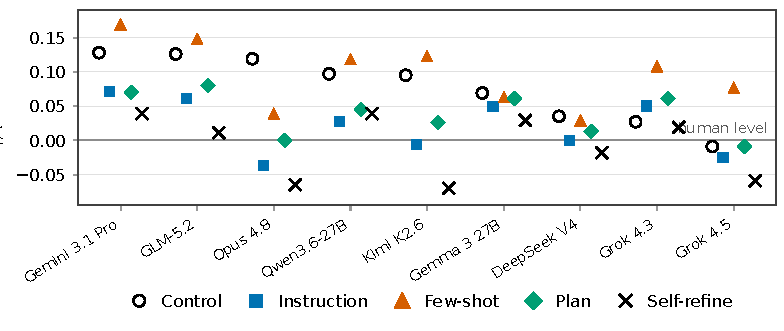
\includegraphics[width=0.95\textwidth,height=5.6cm]{figures/fig_aimscatter.pdf}
\caption{Median $\Delta B_n =$ human $-$ model for every family and prompting mode, the
forty-five cells of Table~\ref{tab:ninefam}. Reading key: the gray line is the human dispersion
level; markers above it are flatter than the human articles, markers below it more dispersed.
Families are ordered by their control-mode gap. Every control marker except Grok 4.5's sits
above the line, few-shot sits highest in six of nine families by median, and is the flattest mode by rank-biserial in seven: the difference is Gemma 3 27B, where few-shot carries the larger effect size but control the larger median, and instruction lands on both
sides of the line, including across the three leftmost families whose control markers nearly
coincide. Per-cell significance is in Table~\ref{tab:ninefam}.}
\label{fig:aimscatter}
\end{figure}

Table~\ref{tab:ninefam} reports the $B_n$ cell for every mode on every family,
Figure~\ref{fig:aimscatter} plots all forty-five cells, and
Appendix~\ref{sec:familygrids} carries each family's full four-dimension grid with its
correction census.

Uninstructed, eight of nine families write significantly flatter than the human articles,
with control deficits from $0.027$ to $0.128$. Grok 4.5's control-mode difference is not
significant ($-0.009$, $p=0.086$). The three largest gaps belong to the frontier flagships, Gemini 3.1 Pro
($0.128$, rank-biserial $0.85$), GLM-5.2 ($0.126$, $0.85$), and Claude Opus 4.8 ($0.119$,
$0.80$), which start within $0.009$ of one another, so frontier scale alone does not close
the gap. Deficits of at most $0.128$ on a coefficient bounded in $[-1,1]$ are consistent
signatures, well short of the gross flatness the detector literature
describes~\citep{arxiv2024detecting}.

On four families the instruction narrows the gap without closing it: Gemini 3.1 Pro lands
at $0.071$, GLM-5.2 at $0.061$, Qwen3.6-27B at $0.028$, and Gemma 3 27B at $0.049$.

Two families land on the human dispersion level, and we state both as CI-bounded
equivalence with pre-specified margins. DeepSeek V4 Pro closes a significant control gap
($0.035$, rank-biserial $0.34$, $p=3\times10^{-5}$) to a median delta of $0.000$ with
$95\%$ CI $[-0.012, 0.026]$ ($p=0.57$), inside the tightest margin, $m^{*}=0.026$.
Kimi K2.6 closes $0.095$ ($0.69$) to $-0.006$ with CI $[-0.034, 0.020]$ ($p=0.96$),
bounded at the middle margin, $m^{*}=0.034$. The DeepSeek landing is one-dimensional: its instructed leg overshoots
human segmentation entropy ($-0.145$, rank-biserial $-0.47$, $p<10^{-5}$) while matching
dispersion. Kimi's instructed leg shows no per-cell significant difference on any
dimension, though only its dispersion cell carries an equivalence bound.

Five of the forty-five cells land significantly past the human articles. Claude Opus 4.8 and
Grok 4.5 cross under instruction ($-0.037$, rank-biserial $-0.25$, $p=0.002$, surviving both
corrections; $-0.025$, $-0.20$, $p=0.015$, surviving Benjamini--Hochberg, falling under Holm),
and self-refine pushes three families past (Kimi K2.6 $-0.070$, Claude Opus 4.8 $-0.065$,
Grok 4.5 $-0.059$, all surviving both corrections). Instruction widens Grok 4.3's gap from
$0.027$ to $0.050$ (the modes' CIs overlap, $[0.005, 0.044]$ and $[0.030, 0.068]$), and
Grok 4.5, one generation later, inverts past the human level. The flatness tell is not
monotone even within a single vendor.

The identical instruction lands Gemini 3.1 Pro, GLM-5.2, and Claude Opus 4.8 at $0.071$,
$0.061$, and $-0.037$, two significantly short of the human articles and one significantly
past them. The wording alone moves Claude Opus 4.8 from significantly short of the human
articles in control and few-shot to significantly past them under instruction and self-refine.

All nine families undershoot significantly under few-shot. The few-shot gap exceeds the
family's control gap in six of nine, and ranked by rank-biserial it is the largest-effect
mode in seven of nine ($0.94$ on Gemini 3.1 Pro and GLM-5.2, $0.83$ on Kimi K2.6, $0.80$
on Qwen3.6-27B, $0.76$ on Grok 4.3, $0.69$ on Grok 4.5, $0.65$ on Gemma 3 27B). The
exceptions, DeepSeek V4 Pro and Claude Opus 4.8, are the families whose uninstructed
control carries the larger effect. On Grok 4.5 few-shot alone drags the model back below
the human level ($0.077$, rank-biserial $0.69$, $p<10^{-5}$). The exemplars are three
human news reports at the median of the human rhythm distribution
(Appendix~\ref{sec:prompts}), so showing the model typical human rhythm produces text
farther from it than saying nothing, in six of nine families; one reading we did not
test is register reproduction rather than variance.

The synthesis is the scatter. Across the forty-five family-by-mode cells, thirty-two land
significantly flatter than the human articles, eight show no significant difference, and five
land significantly more dispersed. The same instruction, word for word, leaves four families
significantly short of the human dispersion level, lands two on it, moves one further away, and
pushes two significantly past. Prompt-level control has poor aim: its gain and even its sign are
family-dependent, and the uninstructed gap does not predict the landing. This is what the
diagnostic exposes: the gap it measures cannot be closed reliably from the prompt side, because
the instruction that reaches parity on one family moves the next one a different amount and
sometimes the wrong way.

\section{Discussion}\label{sec:discussion}

\paragraph{What this audit prescribes for evaluation practice.}
\begin{enumerate}\setlength{\itemsep}{2pt}\setlength{\parsep}{0pt}\setlength{\topsep}{4pt}
\item Normalize before scoring: any segmenter-based feature computed on raw model output measures formatting as well as rhythm, and the unreported choice can flip verdicts in both directions (Section~\ref{sec:normalization}).
\item Sample multiple seeds and average within headline before testing: pooling seeds pseudo-replicates the human baseline and overstates significance (Section~\ref{sec:analysis}).
\item Audit empty cells: silent provider moderation returns ordinary responses with empty output, and unlogged empties reshape scores invisibly (Section~\ref{sec:ninefam}).
\item State parity as CI-bounded equivalence against pre-specified margins and report the smallest margin cleared; a failure to reject is not a match (Section~\ref{sec:analysis}).
\end{enumerate}

\paragraph{Trusting burstiness as a detection signal.}
Because burstiness is the feature detectors lean on, a definition that raises it could be read as an anti-detection tool. We resist that framing on scientific and ethical grounds. For generation, the plain instruction's landing is family-dependent, significantly short of the human dispersion level on five of nine families, on it on two, and past it on two. For detection, the instructed dispersion signature persists in five of nine families, but Grok 4.5, Kimi K2.6, and Claude Opus 4.8 each write at or beyond human dispersion under at least one prompted mode, where a flatness threshold fires in the wrong direction, and any segmenter-based feature computed on raw output inherits the formatting artifacts of Section~\ref{sec:normalization}. We report detector-relevant behavior across the construct rather than optimizing to defeat any one detector, and the strong detector signal (surprisal) stays outside it.

\paragraph{Dual use and disclosure.}
We disclose AI-assisted research per the venue policy, and we benchmark against detectors transparently.

\paragraph{What the diagnostic leaves open.}
For the five modes tested, the landing cannot be aimed: the same wording lands families short of, on, and past the human level, and the uninstructed gap does not predict which.

\section{Limitations}\label{sec:limitations}

\paragraph{Limits of the metric.}
Statistical separation is not construct validity: significant paired
differences show the coefficient separates authorship in matched news prose, and they leave open
whether it captures everything meant by rhythm.
The coefficient $B_n$ inherits the weaknesses of the coefficient of variation it reparametrizes
(Section~\ref{sec:formalizing}): it is order-blind and shape-blind,
scoring the dispersion of the length sequence while ignoring where the long and short sentences fall, and memory recovers only
lag-1 order. Surprisal is model-relative, which is why it stays outside the construct and is
not scored. The metric is unreliable below its ten-sentence floor
(Section~\ref{sec:formalizing}) and is genre-relative: target bands do not transfer unchanged
across registers. Syntactic complexity, a second intended axis of structural
variation, is work in progress and not part of the locked definition. Guard thresholds are heuristic: they set a floor and prove nothing about
strategies outside their list.

\paragraph{Limits of the experiment.}
The corpus is a single register (Wikinews, expository news, English), chosen as a
conservative, low-rhythm register, so reported gaps are likely smaller than on narrative
or literary text. Nine families occupy a narrow band of contemporary instruction-tuned assistants, the
Grok pair contributing two successive generations; for budget reasons we omitted an OpenAI
leg. Results are not yet shown across genres, languages, or future vintages, and burstiness norms are themselves genre- and language-relative. The flatness tell is model- and vintage-relative: Grok 4.3 to
Grok 4.5 flips the instruction-mode gap in a single generation, so the gaps we measure should not be read as constants of nature. One fixed wording per mode risks measuring one model's reading of one
prompt. Cross-family replication removes part of that risk, since few-shot is the
largest-effect mode by rank-biserial in seven of nine families (DeepSeek V4 Pro and Claude Opus 4.8 are the
exceptions). DeepSeek V4 Pro's three metric-free paraphrases land instruction at or past the
human articles on $B_n$ (median deltas $-0.026$ to $-0.030$ against the canonical wording's
$+0.000$), so the mode conclusion holds under rewording, with a wording-sensitivity band of
about $0.03$.

Decoding is not matched across providers (four legs do not honor a temperature setting,
two ran at provider defaults, one closed leg ran at temperature $1.0$), so cross-family
magnitude comparisons carry a decoding confound while within-family comparisons do not,
since every mode of a leg ran under the same decoding.
Each twenty-cell grid receives a Benjamini--Hochberg correction
(Appendix~\ref{sec:familygrids}), and no correction spans families. Of the five past-human
cells, four survive both corrections; Grok 4.5's instruction inversion is exploratory under
Holm. Where we claim equivalence we bound it, but the margins are analysis-time
choices: $0.03$ on a $[-1,1]$ coefficient is a judgment about practical
insignificance.

The human articles may appear in the generators' training data: the 2016--2021 corpus predates all nine training cutoffs; we measured overlap directly.
An $n$-gram probe over $600$ control-mode generations per model on three families finds
mean matched 8-gram overlap with the paired article of $0.00055$ (Qwen3.6-27B, max $0.036$),
$0.00207$ (DeepSeek V4 Pro, max $0.104$), and $0.00098$ (Grok 4.3, max $0.062$), against a
mismatched-article baseline mean of $0.0$ everywhere; 13-gram means are at or below $0.00064$ for
all three. The worst single generation shares roughly
$10\%$ of its 8-grams with its paired article, consistent with a shared quotation rather
than memorization. Verbatim reproduction therefore cannot explain the measured gaps on the
probed families. Memorization would move dispersion toward the human level, so any unprobed
effect, whether a deficit or an overshoot, is, if contaminated, an underestimate. The direction reverses for the parity landings:
memorization would inflate instructed dispersion to the human level, so contamination could manufacture the equivalences we report. Both fall in the instruction
mode the probe did not cover; DeepSeek V4 Pro's control-mode overlap ($0.00207$) bounds it only indirectly, and the
probe did not cover Kimi K2.6 at all.

\section{Conclusion}
Burstiness has been measured everywhere and, in detection practice, formalized only in an
unreviewed detector note. This paper gives it a reproducible, model-free definition
hardened against gaming, and surprisal stays outside. Its first use is the aim problem: on
uniformly normalized text, eight of nine families write significantly flatter than the
human articles uninstructed. The same instruction leaves four families significantly short
of the human dispersion level, lands two on it, moves one further away, and pushes two
significantly past it. Few-shot exemplars are the flattest mode by rank-biserial in seven of nine.

The contribution is the composition: a principled, model-free
definition, guarded against gaming, scored on uniformly normalized text,
and exercised in a matched paired design across nine families.
The gap it exposes is one that prompting moves but cannot reliably
close.

\bibliographystyle{plainnat}
\bibliography{references}

\appendix

\section{Prompt wordings}
\label{sec:prompts}

The five prompting modes share one length-matched task brief and, apart from the control mode,
one persona frame. This appendix gives the exact wording of every component, the rule that
composes them into each mode, and two rules the wording leaves implicit: how the target length is
set and how the few-shot exemplars are chosen. The byte-exact source is \path{bench/prompts.py}
in the released code, which also carries a self-check that enforces the three-call structure of
the self-refine mode and the metric-free property stated below. In the blocks that follow, lines
beginning with \texttt{\#} are annotations; every other line is the literal prompt string, with
the long single-line strings wrapped to fit the page and blank lines marking the paragraph breaks
inside a string. Braced tokens such as \texttt{\{headline\}} are filled per generation.

\begin{verbatim}
# BRIEF: control mode sends only this
Write a news article with the following headline:

{headline}

Aim for about {target_words} words.

# VOICE: prepended to every non-control mode
Act as a professional news journalist. Provide the article a seasoned
staff reporter would write: concrete and specific, in a natural human
voice, never flat or mechanical.

# TAIL: appended to every non-control mode
Keep that natural, human quality all the way through, including the
closing paragraphs.

# PLAN: plan-mode body, between VOICE and BRIEF
Before you write, plan the article the way a reporter does: pick the
lede (the single most important fact), then lay out the who, what,
when, where, why, and how, and the order to present them, most
important first. Work that outline out for yourself, then write the
article to it. Do not show your planning; return only the finished
article.

# FEWSHOT_LEAD / FEWSHOT_TAIL: wrap the exemplar block
Study the voice, pacing, and rhythm of the examples below, then write
in the same spirit. Borrow only their style, never their facts or
wording.

<examples>
<example>
# exemplar 1 (full article text omitted; see "Few-shot exemplars" below)
</example>
# ... two more <example> blocks, three exemplars in total ...

</examples>

# FEEDBACK: self-refine call 2, over call 1's {draft}
You are a demanding editor. Critique the draft below only on how
naturally human its prose reads: its rhythm, pacing, and flow. Name
at least THREE specific passages that read as flat, monotonous, or
mechanical. For each, quote the exact sentence(s) and say concretely
what to change to give it a more human cadence. Do not rewrite the
draft; give only the critique. Even if the writing is already strong,
still name the three weakest spots.

DRAFT:
{draft}

# REWRITE: self-refine call 3, over {draft} and {feedback}
Here is your draft and an editor's critique.

DRAFT:
{draft}

CRITIQUE:
{feedback}

Rewrite the article in full, applying every point of the critique. This
is a substantial rewrite, not a light edit: change how the sentences
move wherever the critique flagged flatness, while preserving the
meaning, the facts, and the target length. Return only the rewritten
article.
\end{verbatim}

\paragraph{How the modes compose.} The control mode sends the bare brief and nothing else. Every
other mode follows one template: the voice preamble, then a mode-specific body, then the same
brief, then the tail. The plain instruction has an empty body, so it reduces to the voice
preamble, the brief, and the tail. The plan mode puts the plan text in the body slot, and the
few-shot mode puts the exemplar block there. Self-refine is three model calls on a single
article: a draft from the instruction prompt, a critique from the feedback prompt applied to that
draft, and a rewrite from the rewrite prompt applied to the draft and the critique. A self-check
in \path{bench/prompts.py} asserts the three calls.

\paragraph{Length brief.} The \texttt{\{target\_words\}} slot is the paired human article's word
count rounded to the nearest $25$, so every generation targets its human counterpart's length
(Section~\ref{sec:corpus}).

\paragraph{Few-shot exemplars.} The exemplar block holds three straight news reports drawn from
Wikinews articles outside the $200$ evaluation set. They are the reports whose burstiness sits
nearest the median of the human distribution, chosen for register and topic. The selection uses
$B_n$ only to locate that median and drop degenerate tails, never to pick high-dispersion
exemplars, so the few-shot condition sees typical human rhythm and no exemplar is chosen to teach
to the test. Their full texts are
committed with the released code and are omitted here for length.

\paragraph{Metric-free wording.} None of the prompts names the axis the benchmark scores. A
self-check enforces that no prompt string contains a measured-axis term, among them
\emph{burstiness}, \emph{sentence length}, \emph{variance}, and \emph{standard deviation}. No
prompt gives the model a numeric target on a measured axis; the word count in the length brief is
a length target only. Keeping the axis out of the wording guards against teaching to
the test.

\paragraph{Instruction paraphrases (wording-robustness probe).} The probe in
Section~\ref{sec:limitations} re-runs the instruction mode on DeepSeek V4 Pro under three
independent rewrites of the voice and tail above, one seed over all $200$ briefs, each keeping the
persona frame and the metric-free property. The harness is
\path{experiments/ablation/prompt_paraphrase.py}. The three pairs follow, the voice prepended and
the tail appended around the same brief.

\begin{verbatim}
# PARAPHRASE v1 (VOICE then TAIL)
You are a veteran newspaper reporter. Write the story the way
an experienced newsroom professional would: specific, grounded
in facts, with a voice that reads as unmistakably human rather
than machine-written.

Hold that authentic reporter's voice through to the final sentence.

# PARAPHRASE v2 (VOICE then TAIL)
Take the role of a seasoned journalist at a major daily. Produce
the kind of article an editor would run with light touches only:
concrete details, a living, natural voice, nothing stiff or
formulaic.

Make sure the writing still sounds fully human in the closing
paragraphs, not just the opening.

# PARAPHRASE v3 (VOICE then TAIL)
Write as a long-time staff correspondent. The article should
carry the texture of real human reportage: precise facts,
natural phrasing, and none of the flat, mechanical quality of
generated text.

Sustain that human texture to the very end of the piece.
\end{verbatim}

\section{Per-family result grids}\label{sec:familygrids}

Every family ran the identical full design: the same $200$ matched headlines, the same five
mode wordings (Appendix~\ref{sec:prompts}), three seeds, uniform normalization, and the same
paired scoring on all four dimensions. Qwen3.6-27B's grid is Table~\ref{tab:promptceiling}, and the eight
grids that follow complete the set,
generated from each family's released evaluation with no hand-transcribed values. Within each
family we apply Benjamini--Hochberg at $q=0.05$ across its twenty cells and report the census in
the caption, with the stricter Holm count alongside, and no correction is applied across
families. Instruction-mode equivalence margins are released for every family with the evaluation
artifacts. The two families whose instruction-mode $B_n$ CI clears a pre-specified margin are
DeepSeek V4 Pro ($0.03$) and Kimi K2.6 ($0.05$) (Section~\ref{sec:ninefam}); Kimi's instructed
leg shows no per-cell significant difference on any dimension, though only its dispersion cell
carries an equivalence bound.
Memory $M$ is where three few-shot legs (Qwen3.6-27B, Kimi K2.6, Claude Opus 4.8)
overshoot the human articles even as their dispersion stays significantly flat. Seg.\ entropy, the
axis most exposed to formatting artifacts, still separates on normalized text: instructed
DeepSeek V4 Pro and four of Grok 4.5's five modes sit significantly above the human articles.

\begin{table}[t]
\centering
\caption{Qwen3.6-27B, full grid (uniformly normalized scoring):
seed-averaged Wilcoxon signed-rank paired tests over $200$ matched
headlines per mode. Reading key: median $\Delta =$ human $-$ model; positive means the model is
\emph{below} the
human article on that dimension, the flatness direction. Matched rank-biserial in parentheses;
$^{*}p<0.05$, $^{**}p<0.01$ (per-cell, two-sided). Within-family census: $13$ of $20$ cells
per-cell significant; $12$ survive both Benjamini--Hochberg at $q=0.05$ and Holm (the exception,
instruction-mode memory, is exploratory; Section~\ref{sec:analysis}).}
\label{tab:promptceiling}
\begin{tabular}{lcccc}
\toprule
Mode & $B_n$ & Gini & Seg.\ entropy & Memory $M$ \\
\midrule
Control & $0.097\;(0.67)^{**}$ & $0.046\;(0.67)^{**}$ & $-0.001\;(0.10)$ & $-0.007\;(-0.05)$ \\
Instruction & $0.028\;(0.34)^{**}$ & $0.010\;(0.28)^{**}$ & $-0.018\;(-0.04)$ & $-0.052\;(-0.16)^{*}$ \\
Few-shot & $0.119\;(0.80)^{**}$ & $0.060\;(0.79)^{**}$ & $0.127\;(0.47)^{**}$ & $-0.071\;(-0.26)^{**}$ \\
Plan & $0.045\;(0.41)^{**}$ & $0.017\;(0.35)^{**}$ & $0.057\;(0.16)$ & $-0.028\;(-0.07)$ \\
Self-refine & $0.039\;(0.26)^{**}$ & $0.021\;(0.24)^{**}$ & $0.029\;(0.10)$ & $0.028\;(0.09)$ \\
\bottomrule
\end{tabular}
\end{table}

Table~\ref{tab:promptceiling} reports Qwen3.6-27B's paired deltas. The uninstructed control differs from the human articles where dispersion is
measured: median $\Delta B_n = 0.097$ (rank-biserial $0.67$, $p<10^{-5}$), with Gini concurring
($0.046$, rank-biserial $0.67$). On segmentation entropy ($-0.001$, $p=0.24$) and memory ($-0.007$,
$p=0.52$) the control mode shows no significant difference. The control-mode authorship gap is
confined to the dispersion dimensions.

A plain instruction narrows the dispersion gap by roughly seven tenths and does not close it.
$\Delta B_n$ falls from $0.097$ to $0.028$ (rank-biserial $0.34$, $p=3\times10^{-5}$) and Gini from
$0.046$ to $0.010$ ($p<10^{-3}$); both effects survive correction. Against the
equivalence margins, instruction-mode $B_n$ is not equivalent at $0.03$ (CI $[0.013, 0.046]$,
$m^{*}=0.046$) and becomes equivalent only at $0.05$. Gini is equivalent at $0.03$ ($m^{*}=0.024$),
segmentation entropy at $0.08$ ($m^{*}=0.063$, CI $[-0.063, 0.045]$), and memory at no margin we
test ($m^{*}=0.095$, CI $[-0.095, -0.003]$), though its per-cell significance is the one
exploratory cell of Section~\ref{sec:analysis}.

Few-shot exemplars are the flattest mode on the dispersion statistics, a $B_n$ deficit of $0.119$
with rank-biserial $0.80$, and the per-seed effect holds at $0.724$--$0.745$ on every individual
seed.

Plan and self-refine behave like weaker instructions: significant dispersion deficits ($B_n$
$0.045$ and $0.039$, rank-biserial $0.41$ and $0.26$, both $p<0.01$) with no correction-surviving
effect on segmentation entropy (plan $0.057$, $p=0.052$; self-refine $0.029$, $p=0.22$) or memory.
All ten dispersion cells (five modes by $B_n$ and Gini) are significant at
$p<0.01$ and survive correction, and the only other survivors are few-shot's segmentation
entropy ($0.127$) and memory ($-0.071$) cells.

% Generated by paper/gen_bench_table.py (family grid gemini-3.1-pro) -- do not hand-edit.
\begin{table}[htbp]
\centering
\small
\caption{Gemini 3.1 Pro, full grid: seed-averaged Wilcoxon paired tests over $200$ matched headlines per mode; median $\Delta =$ human $-$ model, matched rank-biserial in parentheses; $^{*}p<0.05$, $^{**}p<0.01$ per cell. Within-family census: $16$ of $20$ cells per-cell significant; all $16$ survive Benjamini--Hochberg at $q=0.05$ ($13$ survive Holm).}
\label{tab:grid-gemini-31-pro}
\begin{tabular}{lcccc}
\toprule
Mode & $B_n$ & Gini & Seg.\ entropy & Memory $M$ \\
\midrule
Control & $0.128\;(0.85)^{**}$ & $0.056\;(0.81)^{**}$ & $-0.062\;(-0.19)^{*}$ & $0.043\;(0.18)^{*}$ \\
Instruction & $0.071\;(0.56)^{**}$ & $0.026\;(0.47)^{**}$ & $-0.053\;(-0.16)$ & $0.109\;(0.38)^{**}$ \\
Few-shot & $0.169\;(0.94)^{**}$ & $0.080\;(0.93)^{**}$ & $0.117\;(0.39)^{**}$ & $0.051\;(0.24)^{**}$ \\
Plan & $0.070\;(0.58)^{**}$ & $0.028\;(0.48)^{**}$ & $-0.026\;(-0.06)$ & $0.114\;(0.47)^{**}$ \\
Self-refine & $0.039\;(0.27)^{**}$ & $0.013\;(0.21)^{**}$ & $-0.051\;(-0.12)$ & $0.047\;(0.12)$ \\
\bottomrule
\end{tabular}
\end{table}

% Generated by paper/gen_bench_table.py (family grid gemma-3-27b) -- do not hand-edit.
\begin{table}[htbp]
\centering
\small
\caption{Gemma 3 27B, full grid (design and conventions as in Table~\ref{tab:promptceiling}: median $\Delta =$ human $-$ model, matched rank-biserial in parentheses; $^{*}p<0.05$, $^{**}p<0.01$ per cell). Within-family census: $16$ of $20$ cells per-cell significant; all $16$ survive both Benjamini--Hochberg at $q=0.05$ and Holm.}
\label{tab:grid-gemma-3-27b}
\begin{tabular}{lcccc}
\toprule
Mode & $B_n$ & Gini & Seg.\ entropy & Memory $M$ \\
\midrule
Control & $0.069\;(0.58)^{**}$ & $0.037\;(0.58)^{**}$ & $0.063\;(0.25)^{**}$ & $0.023\;(0.11)$ \\
Instruction & $0.049\;(0.44)^{**}$ & $0.025\;(0.41)^{**}$ & $0.086\;(0.36)^{**}$ & $0.040\;(0.10)$ \\
Few-shot & $0.063\;(0.65)^{**}$ & $0.033\;(0.63)^{**}$ & $0.145\;(0.48)^{**}$ & $0.005\;(0.02)$ \\
Plan & $0.061\;(0.57)^{**}$ & $0.033\;(0.55)^{**}$ & $0.129\;(0.45)^{**}$ & $0.003\;(0.03)$ \\
Self-refine & $0.029\;(0.30)^{**}$ & $0.015\;(0.29)^{**}$ & $0.094\;(0.32)^{**}$ & $0.048\;(0.21)^{**}$ \\
\bottomrule
\end{tabular}
\end{table}

% Generated by paper/gen_bench_table.py (family grid deepseek-v4-pro) -- do not hand-edit.
\begin{table}[htbp]
\centering
\small
\caption{DeepSeek V4 Pro, full grid (design and conventions as in Table~\ref{tab:promptceiling}: median $\Delta =$ human $-$ model, matched rank-biserial in parentheses; $^{*}p<0.05$, $^{**}p<0.01$ per cell). Within-family census: $8$ of $20$ cells per-cell significant; all $8$ survive Benjamini--Hochberg at $q=0.05$ ($6$ survive Holm). The instruction-mode $B_n$ cell is the CI-bounded equivalence result of Section~\ref{sec:ninefam}.}
\label{tab:grid-deepseek-v4-pro}
\begin{tabular}{lcccc}
\toprule
Mode & $B_n$ & Gini & Seg.\ entropy & Memory $M$ \\
\midrule
Control & $0.035\;(0.34)^{**}$ & $0.018\;(0.35)^{**}$ & $-0.050\;(-0.12)$ & $-0.025\;(-0.07)$ \\
Instruction & $0.000\;(0.05)$ & $-0.005\;(-0.02)$ & $-0.145\;(-0.47)^{**}$ & $0.006\;(0.07)$ \\
Few-shot & $0.029\;(0.24)^{**}$ & $0.014\;(0.20)^{*}$ & $-0.068\;(-0.26)^{**}$ & $0.012\;(0.01)$ \\
Plan & $0.013\;(0.15)$ & $0.003\;(0.08)$ & $-0.117\;(-0.36)^{**}$ & $-0.003\;(0.03)$ \\
Self-refine & $-0.018\;(-0.10)$ & $-0.010\;(-0.11)$ & $-0.139\;(-0.49)^{**}$ & $0.027\;(0.14)$ \\
\bottomrule
\end{tabular}
\end{table}

% Generated by paper/gen_bench_table.py (family grid grok-4.3) -- do not hand-edit.
\begin{table}[htbp]
\centering
\small
\caption{Grok 4.3, full grid (design and conventions as in Table~\ref{tab:promptceiling}: median $\Delta =$ human $-$ model, matched rank-biserial in parentheses; $^{*}p<0.05$, $^{**}p<0.01$ per cell). Within-family census: $13$ of $20$ cells per-cell significant; all $13$ survive Benjamini--Hochberg at $q=0.05$ ($9$ survive Holm).}
\label{tab:grid-grok-43}
\begin{tabular}{lcccc}
\toprule
Mode & $B_n$ & Gini & Seg.\ entropy & Memory $M$ \\
\midrule
Control & $0.027\;(0.27)^{**}$ & $0.010\;(0.23)^{**}$ & $-0.046\;(-0.16)$ & $-0.004\;(0.01)$ \\
Instruction & $0.050\;(0.42)^{**}$ & $0.026\;(0.39)^{**}$ & $0.062\;(0.19)^{*}$ & $0.028\;(0.10)$ \\
Few-shot & $0.108\;(0.76)^{**}$ & $0.052\;(0.74)^{**}$ & $0.180\;(0.56)^{**}$ & $0.001\;(-0.05)$ \\
Plan & $0.061\;(0.56)^{**}$ & $0.026\;(0.50)^{**}$ & $0.136\;(0.35)^{**}$ & $0.023\;(0.03)$ \\
Self-refine & $0.019\;(0.19)^{*}$ & $0.009\;(0.14)$ & $0.055\;(0.21)^{**}$ & $0.028\;(0.14)$ \\
\bottomrule
\end{tabular}
\end{table}

% Generated by paper/gen_bench_table.py (family grid grok-4.5) -- do not hand-edit.
\begin{table}[htbp]
\centering
\small
\caption{Grok 4.5, full grid (design and conventions as in Table~\ref{tab:promptceiling}: median $\Delta =$ human $-$ model, matched rank-biserial in parentheses; $^{*}p<0.05$, $^{**}p<0.01$ per cell). Negative cells place the model above the human articles, more dispersed than the human baseline. Within-family census: $14$ of $20$ cells per-cell significant; $13$ survive Benjamini--Hochberg at $q=0.05$ (control-mode Gini, $p=0.037$, is the loss; $9$ survive Holm).}
\label{tab:grid-grok-45}
\begin{tabular}{lcccc}
\toprule
Mode & $B_n$ & Gini & Seg.\ entropy & Memory $M$ \\
\midrule
Control & $-0.009\;(-0.14)$ & $-0.011\;(-0.17)^{*}$ & $-0.249\;(-0.74)^{**}$ & $-0.023\;(-0.07)$ \\
Instruction & $-0.025\;(-0.20)^{*}$ & $-0.014\;(-0.20)^{*}$ & $-0.099\;(-0.40)^{**}$ & $0.048\;(0.22)^{**}$ \\
Few-shot & $0.077\;(0.69)^{**}$ & $0.039\;(0.68)^{**}$ & $0.089\;(0.28)^{**}$ & $-0.002\;(-0.05)$ \\
Plan & $-0.009\;(-0.02)$ & $-0.005\;(-0.05)$ & $-0.062\;(-0.22)^{**}$ & $0.021\;(0.06)$ \\
Self-refine & $-0.059\;(-0.41)^{**}$ & $-0.033\;(-0.44)^{**}$ & $-0.133\;(-0.44)^{**}$ & $0.071\;(0.31)^{**}$ \\
\bottomrule
\end{tabular}
\end{table}

% Generated by paper/gen_bench_table.py (family grid glm-5.2) -- do not hand-edit.
\begin{table}[htbp]
\centering
\small
\caption{GLM-5.2, full grid (design and conventions as in Table~\ref{tab:promptceiling}: median $\Delta =$ human $-$ model, matched rank-biserial in parentheses; $^{*}p<0.05$, $^{**}p<0.01$ per cell). Within-family census: $16$ of $20$ cells per-cell significant; $16$ survive Benjamini--Hochberg at $q=0.05$ ($14$ survive Holm). 36 silent-refusal empty cells are excluded by the seed-averaging protocol (Section~\ref{sec:ninefam}).}
\label{tab:grid-glm-52}
\begin{tabular}{lcccc}
\toprule
Mode & $B_n$ & Gini & Seg.\ entropy & Memory $M$ \\
\midrule
Control & $0.126\;(0.85)^{**}$ & $0.058\;(0.82)^{**}$ & $0.068\;(0.25)^{**}$ & $0.053\;(0.19)^{*}$ \\
Instruction & $0.061\;(0.57)^{**}$ & $0.029\;(0.51)^{**}$ & $0.064\;(0.26)^{**}$ & $0.076\;(0.24)^{**}$ \\
Few-shot & $0.148\;(0.94)^{**}$ & $0.068\;(0.92)^{**}$ & $0.221\;(0.74)^{**}$ & $0.022\;(0.07)$ \\
Plan & $0.080\;(0.65)^{**}$ & $0.034\;(0.59)^{**}$ & $0.091\;(0.32)^{**}$ & $0.034\;(0.20)^{*}$ \\
Self-refine & $0.011\;(0.13)$ & $0.002\;(0.09)$ & $0.050\;(0.33)^{**}$ & $-0.019\;(-0.02)$ \\
\bottomrule
\end{tabular}
\end{table}

% Generated by paper/gen_bench_table.py (family grid kimi-k2.6) -- do not hand-edit.
\begin{table}[htbp]
\centering
\small
\caption{Kimi K2.6, full grid (design and conventions as in Table~\ref{tab:promptceiling}: median $\Delta =$ human $-$ model, matched rank-biserial in parentheses; $^{*}p<0.05$, $^{**}p<0.01$ per cell). Within-family census: $12$ of $20$ cells per-cell significant; $10$ survive Benjamini--Hochberg at $q=0.05$ ($9$ survive Holm). 25 provider content-filter refusals are excluded by the seed-averaging protocol (Section~\ref{sec:ninefam}).}
\label{tab:grid-kimi-k26}
\begin{tabular}{lcccc}
\toprule
Mode & $B_n$ & Gini & Seg.\ entropy & Memory $M$ \\
\midrule
Control & $0.095\;(0.69)^{**}$ & $0.043\;(0.63)^{**}$ & $-0.048\;(-0.16)^{*}$ & $-0.025\;(-0.09)$ \\
Instruction & $-0.006\;(-0.00)$ & $-0.014\;(-0.14)$ & $-0.024\;(-0.11)$ & $-0.014\;(0.08)$ \\
Few-shot & $0.123\;(0.83)^{**}$ & $0.063\;(0.79)^{**}$ & $0.152\;(0.55)^{**}$ & $-0.073\;(-0.26)^{**}$ \\
Plan & $0.026\;(0.24)^{**}$ & $0.006\;(0.09)$ & $0.032\;(0.05)$ & $0.055\;(0.17)^{*}$ \\
Self-refine & $-0.070\;(-0.57)^{**}$ & $-0.040\;(-0.58)^{**}$ & $0.061\;(0.16)$ & $-0.052\;(-0.23)^{**}$ \\
\bottomrule
\end{tabular}
\end{table}

% Generated by paper/gen_bench_table.py (family grid opus-4.8) -- do not hand-edit.
\begin{table}[htbp]
\centering
\small
\caption{Claude Opus 4.8, full grid (design and conventions as in Table~\ref{tab:promptceiling}: median $\Delta =$ human $-$ model, matched rank-biserial in parentheses; $^{*}p<0.05$, $^{**}p<0.01$ per cell). Within-family census: $16$ of $20$ cells per-cell significant; $16$ survive Benjamini--Hochberg at $q=0.05$ ($15$ survive Holm). Ran at effort high with a 32{,}000-token cap; both deviations and their measurements are recorded in the leg metadata (Section~\ref{sec:ninefam}).}
\label{tab:grid-opus-48}
\begin{tabular}{lcccc}
\toprule
Mode & $B_n$ & Gini & Seg.\ entropy & Memory $M$ \\
\midrule
Control & $0.119\;(0.80)^{**}$ & $0.054\;(0.77)^{**}$ & $0.116\;(0.39)^{**}$ & $-0.069\;(-0.24)^{**}$ \\
Instruction & $-0.037\;(-0.25)^{**}$ & $-0.031\;(-0.36)^{**}$ & $0.032\;(0.09)$ & $-0.117\;(-0.38)^{**}$ \\
Few-shot & $0.039\;(0.34)^{**}$ & $0.012\;(0.26)^{**}$ & $0.253\;(0.75)^{**}$ & $-0.045\;(-0.25)^{**}$ \\
Plan & $-0.000\;(0.01)$ & $-0.004\;(-0.10)$ & $0.108\;(0.34)^{**}$ & $-0.059\;(-0.25)^{**}$ \\
Self-refine & $-0.065\;(-0.50)^{**}$ & $-0.043\;(-0.59)^{**}$ & $-0.005\;(0.01)$ & $0.039\;(0.18)^{*}$ \\
\bottomrule
\end{tabular}
\end{table}

\begin{figure}[t]
\centering
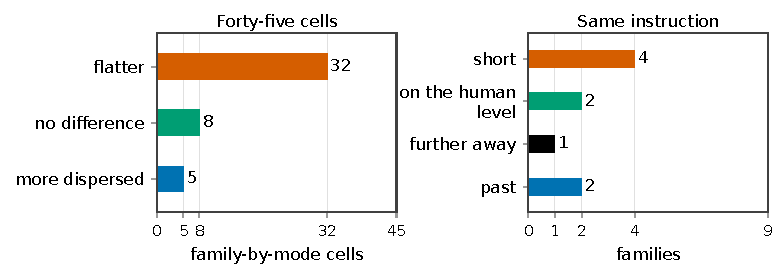
\includegraphics[width=0.95\textwidth,height=4.6cm]{figures/fig_landings.pdf}
\caption{Left: of the forty-five family-by-mode cells, thirty-two land
significantly flatter than the human articles, eight show no significant
difference, and five land significantly more dispersed. Right: the same
instruction leaves four families significantly short of the human
dispersion level, lands two on it, moves one further away, and pushes two
significantly past (Section~\ref{sec:ninefam}).}
\label{fig:landings}
\end{figure}

\section{Reference implementation}
\label{sec:refimpl}

The measurement instrument is model-free and pure standard library. The listing below is the
complete, self-contained implementation used in this paper: the sentence segmenter, the
burstiness coefficient $B_n$ (Goh--Barab\'asi under the Kim--Jo finite-$n$ correction), the
memory coefficient $M$, the Gini robustness check, Miller--Madow segmentation entropy, the
multiscale profile, and the Goodhart guard, whose thresholds are its default keyword arguments.
It runs on any Python~3 interpreter with no third-party dependencies and no reference model.

\begin{lstlisting}[language=Python]
"""Reference implementation of the burstiness measurement instrument.

Model-free and pure standard library. Segments a document into sentence
lengths and computes the burstiness coefficient B_n (Goh-Barabasi under the
Kim-Jo finite-n correction), the memory coefficient M, the Gini robustness
check, Miller-Madow segmentation entropy, and a multiscale profile. The
Goodhart guard screens degenerate text that would game a dispersion score.
"""
from __future__ import annotations

import math
import re
from statistics import fmean, pstdev
from typing import List, Optional, Sequence

# Below this many sentences, B_n and M estimates are noisy and biased; the
# entry point reports ``reliable = False`` rather than trusting them.
RELIABILITY_FLOOR = 10

# --------------------------------------------------------------------------
# Segmentation: sentence lengths in whitespace tokens (stdlib only)
# --------------------------------------------------------------------------

_ABBREVIATIONS = {
    "mr", "mrs", "ms", "dr", "prof", "sr", "jr", "st", "vs", "etc",
    "e.g", "i.e", "fig", "no", "vol", "cf", "al", "inc", "ltd", "co",
}
_SENT_SPLIT = re.compile(r'([.!?]+["\')\]]?)\s+')
_PUNCT_SYMBOLS = re.compile(r'[.!?,;:\-—()"\']')


def sentence_lengths(text: str) -> List[int]:
    """Word-token count of each sentence, with an abbreviation-guarded split."""
    if not text or not text.strip():
        return []
    sentences: List[str] = []
    last = 0
    for m in _SENT_SPLIT.finditer(text):
        end = m.end()
        candidate = text[last:end].strip()
        bare = candidate.rstrip('.!?"\')]').strip()
        last_word = bare.split()[-1].lower() if bare.split() else ""
        if last_word in _ABBREVIATIONS:
            continue
        if candidate:
            sentences.append(candidate)
        last = end
    tail = text[last:].strip()
    if tail:
        sentences.append(tail)
    return [len(s.split()) for s in sentences if s.split()]


# --------------------------------------------------------------------------
# Core coefficients (operate on a sequence of sentence lengths)
# --------------------------------------------------------------------------

def burstiness_B(intervals: Sequence[float]) -> Optional[float]:
    """Goh-Barabasi coefficient B = (sigma - mu) / (sigma + mu), bounded [-1, 1]."""
    if len(intervals) < 2:
        return None
    mu = fmean(intervals)
    sigma = pstdev(intervals)
    denom = sigma + mu
    if denom <= 0:
        return None
    return (sigma - mu) / denom


def burstiness_B_corrected(intervals: Sequence[float]) -> Optional[float]:
    """Kim-Jo finite-n correction B_n; reduces to (r-1)/(r+1) as n -> inf."""
    n = len(intervals)
    if n < 2:
        return None
    mu = fmean(intervals)
    if mu <= 0:
        return None
    r = pstdev(intervals) / mu
    sp, sm = math.sqrt(n + 1), math.sqrt(n - 1)
    denom = (sp - 2.0) * r + sm
    if denom == 0:
        return None
    return (sp * r - sm) / denom


def memory_M(intervals: Sequence[float]) -> Optional[float]:
    """Lag-1 autocorrelation of consecutive sentence lengths (the memory term)."""
    n = len(intervals)
    if n < 3:
        return None
    a = list(intervals[:-1])
    b = list(intervals[1:])
    m1, m2 = fmean(a), fmean(b)
    s1, s2 = pstdev(a), pstdev(b)
    if s1 <= 0 or s2 <= 0:
        return None
    cov = fmean((x - m1) * (y - m2) for x, y in zip(a, b))
    return cov / (s1 * s2)


def gini(intervals: Sequence[float]) -> float:
    """Gini coefficient of sentence lengths; scale-free robustness check for B_n."""
    n = len(intervals)
    if n < 2:
        return 0.0
    m = fmean(intervals)
    if m == 0:
        return 0.0
    # Sample (unbiased) Gini: divide by n*(n-1), not n^2, which removes an
    # n-dependent bias that would confound cross-document comparison.
    return sum(abs(a - b) for a in intervals for b in intervals) / (2.0 * n * (n - 1) * m)


_TYPO_QUOTES = str.maketrans({"“": '"', "”": '"', "‘": "'", "’": "'"})


def segmentation_entropy(text: str) -> float:
    """Miller-Madow-corrected Shannon entropy (bits) of the punctuation marks.

    Typographic quotes are normalized to ASCII first, so quote STYLE (curly vs
    straight) is not scored as segmentation diversity.
    """
    counts: dict = {}
    for ch in _PUNCT_SYMBOLS.findall((text or "").translate(_TYPO_QUOTES)):
        counts[ch] = counts.get(ch, 0) + 1
    total = sum(counts.values())
    if total == 0:
        return 0.0
    h = -sum((c / total) * math.log2(c / total) for c in counts.values())
    return h + (len(counts) - 1) / (2.0 * total * math.log(2))


# --------------------------------------------------------------------------
# Multiscale temporal profile
# --------------------------------------------------------------------------

def _coarse_grain(L: Sequence[float], w: int) -> List[float]:
    """Non-overlapping window means: coarsen the length series to scale w."""
    return [fmean(L[i:i + w]) for i in range(0, len(L) - w + 1, w)]


def multiscale_burstiness(text: str, scales: Sequence[int] = (1, 2, 4)) -> dict:
    """B_n at the sentence scale and at coarse-grained window scales.

    Genuine long-range burstiness holds its dispersion at coarse scales, whereas
    mechanical alternation washes out toward B_n = -1 at scale >= 2.
    """
    L = [float(x) for x in sentence_lengths(text)]
    out = {}
    for s in scales:
        cg = list(L) if s == 1 else _coarse_grain(L, s)
        out[f"B_n@{s}"] = burstiness_B_corrected(cg) if len(cg) >= 2 else None
    return out


# --------------------------------------------------------------------------
# Goodhart guard: reject degenerate texts that reach the score by gaming it
# --------------------------------------------------------------------------

def _trigram_diversity(text: str) -> float:
    """Distinct word-trigram ratio (catches verbatim repetition)."""
    w = (text or "").split()
    if len(w) < 4:
        return 1.0
    tris = list(zip(w, w[1:], w[2:]))
    return len(set(tris)) / len(tris)


def _runon_ratio(text: str) -> float:
    """Internal clause delimiters (, ; :) per sentence terminal (. ! ?)."""
    internal = len(re.findall(r"[,;:]", text or ""))
    terminal = len(re.findall(r"[.!?]+", text or "")) or 1
    return internal / terminal


def gaming_flags(text, *, loo_delta=0.25, m_floor=-0.5, m_ceiling=0.7,
                 distinct_len_min=0.5, trigram_min=0.5, frag_frac_max=0.3,
                 punct_rate_max=0.25, runon_max=8.0, finescale_drop=0.4):
    """Flag texts that reach a high dispersion score through degenerate patterns.

    Returns {"ok", "gate_ok", "flags", "detail"}. ``ok`` means no gaming pattern
    fired; ``gate_ok`` means ok AND reliable (n >= RELIABILITY_FLOOR). B_n should
    be counted only when gate_ok is True and a separate coherence gate also
    passes: re-punctuating a fixed text can swing B_n across much of its range,
    so length-rhythm must never select generations on its own.

    Flags: outlier_driven (dropping the longest sentence swings B_n > loo_delta),
    low_len_diversity (distinct-length ratio < distinct_len_min at n >= 8, which
    catches blocky and period-k patterns), repetitive (trigram ratio <
    trigram_min), alternating (M < m_floor), over_clumped (M > m_ceiling),
    fine_scale_only (B_n@1 > 0 but drops by > finescale_drop at scale 2),
    fragment_spam (>= frag_frac_max of sentences under 3 words), punct_gamed
    (punctuation marks per word > punct_rate_max), runon (internal-to-terminal
    delimiter ratio > runon_max).
    """
    Li = [int(x) for x in sentence_lengths(text)]
    L = [float(x) for x in Li]
    n = len(L)
    if n < 3:
        return {"ok": False, "gate_ok": False, "flags": {"too_short": True}, "detail": {"n": n}}

    B_full = burstiness_B_corrected(L)
    j = max(range(n), key=lambda i: L[i])
    B_loo = burstiness_B_corrected(L[:j] + L[j + 1:])
    loo = abs(B_full - B_loo) if (B_full is not None and B_loo is not None) else 0.0
    M = memory_M(L)
    distinct_ratio = len(set(Li)) / n
    trig = _trigram_diversity(text)
    frag_frac = sum(1 for x in Li if x < 3) / n
    words = sum(L) or 1.0
    punct_rate = len(_PUNCT_SYMBOLS.findall(text or "")) / words
    runon = _runon_ratio(text)
    ms = multiscale_burstiness(text)
    b1, b2 = ms.get("B_n@1"), ms.get("B_n@2")
    fine_scale_only = (b1 is not None and b2 is not None and b1 > 0.0
                       and (b1 - b2) > finescale_drop)

    flags = {
        "outlier_driven": loo > loo_delta,
        "low_len_diversity": n >= 8 and distinct_ratio < distinct_len_min,
        "repetitive": trig < trigram_min,
        "alternating": M is not None and M < m_floor,
        "over_clumped": M is not None and M > m_ceiling,
        "fine_scale_only": fine_scale_only,
        "fragment_spam": frag_frac >= frag_frac_max,
        "punct_gamed": punct_rate > punct_rate_max,
        "runon": runon > runon_max,
    }
    ok = not any(flags.values())
    return {
        "ok": ok,
        "gate_ok": ok and n >= RELIABILITY_FLOOR,
        "flags": flags,
        "detail": {"n": n, "loo_dB": round(loo, 3),
                   "M": None if M is None else round(M, 3),
                   "distinct_ratio": round(distinct_ratio, 3), "trigram_div": round(trig, 3),
                   "frag_frac": round(frag_frac, 3), "punct_rate": round(punct_rate, 3),
                   "runon": round(runon, 2)},
    }


# --------------------------------------------------------------------------
# Entry point: the full model-free vector for a document
# --------------------------------------------------------------------------

def burstiness_pp(text: str) -> dict:
    """Model-free structural burstiness of a document.

    B_n is the primary dispersion coefficient, M the lag-1 memory, Gini the
    robustness check, and multiscale the temporal profile. Segmentation entropy
    is a separate axis (see segmentation_entropy) and surprisal is kept outside
    the construct. ``reliable`` is False below RELIABILITY_FLOOR sentences.
    """
    L = [float(x) for x in sentence_lengths(text)]
    n = len(L)
    return {
        "B_n": burstiness_B_corrected(L),
        "M": memory_M(L),
        "gini": gini(L),
        "multiscale": multiscale_burstiness(text),
        "n_sentences": n,
        "reliable": n >= RELIABILITY_FLOOR,
        "sentence_lengths": [int(x) for x in L],
    }
\end{lstlisting}

\section{Protocol and audit detail}\label{sec:protocoldetail}

% Provenance: paper/main.tex lines 294--299
\subsection{Corpus parse mechanics}
The human side of each pair is the plain article body, regenerable from the source Wikinews
wikitext by a deterministic MediaWiki parse (\path{experiments/ablation/clean_wikinews.py})
that keeps the body up to the first section heading or reader-comment block, removes templates,
drops reference tags with their contents, resolves wikilinks to their display text, and unwraps
inline formatting. On a held-out check of $100$ articles this parse reproduces the shipped
human bodies exactly.

% Provenance: paper/main.tex lines 315--319 and 402--412
\subsection{Per-leg completeness}
Completeness is disclosed per leg. Of Qwen3.6-27B's $3{,}000$ cells ($200$ headlines $\times$
$5$ modes $\times$ $3$ seeds), $2{,}996$ completed; we excluded the four that exceeded the
reasoning budget rather than scoring their incomplete output. We average affected headlines
over their remaining seeds, so every mode retains $200$ matched pairs. Grok 4.5 reports two
empty self-refine outputs, truncations by signature, seed-averaged away. Provider content
moderation removes cells on two legs, by two different mechanisms. Moonshot's filter refuses
explicitly: $25$ of Kimi K2.6's $3{,}000$ cells return HTTP $400$, one Hong Kong protest
headline refused at every mode and seed. Zhipu's filter refuses silently: $36$ of GLM-5.2's
cells return an ordinary HTTP $200$ with empty output, concentrated on the same cluster of
politically sensitive headlines. The remaining five legs generated all $200$ headlines in
every mode.

% Provenance: paper/main.tex lines 382--400
\subsection{Per-leg decoding and output caps}
GLM-5.2 ignores a requested temperature and Kimi K2.6 rejects one; Grok 4.5 exposes neither
temperature nor top-$p$; Gemini 3.1 Pro ran at temperature $1.0$ with provider-managed thinking;
Claude Opus 4.8 exposes no temperature. Gemini's thoughts are never returned, and Gemma 3 has
no thinking mode. Anthropic bills reasoning against the output cap. The
shared $16{,}000$-token cap that leaves other families room to write leaves Claude Opus 4.8 with
none at maximum effort: the self-refine rewrite spends the whole budget reasoning. We ran that
leg at high effort with a $32{,}000$-token cap, which restores a comparable prose budget rather
than granting a larger one and matches Gemini 3.1 Pro's thinking level. The leg completed all
$3{,}000$ cells with no truncated or empty output.

% Provenance: paper/main.tex lines 372--374
\subsection{Confidence intervals}
CIs on median paired deltas are percentile bootstrap intervals: the $2.5$th and $97.5$th
percentiles of the medians of $2{,}000$ resamples of the $200$ matched pairs. Per-seed $B_n$
effect sizes are released alongside the evaluation artifacts and are consistent with the
seed-averaged results.

% Provenance: paper/main.tex lines 325--328
\subsection{Scaffolding rates}
A generation-hygiene guard flagged markdown scaffolding and echoed headline blocks in every
family we benchmark, from 23--38\% of control-mode generations on one leg (DeepSeek V4 Pro:
23\% markdown, 38\% title lines) to 100\% on another (Gemma 3 27B markdown; headline echoes on
the Grok 4.5 and Gemini 3.1 Pro legs). All of it is formatting the plain-prose human baseline
lacks.

% Provenance: paper/main.tex lines 680--688
\subsection{Contamination probe values}
An $n$-gram contamination probe over $600$ control-mode generations per model on three families
finds mean matched 8-gram overlap with the paired article of $0.00055$ (Qwen3.6-27B, max
$0.036$), $0.00207$ (DeepSeek V4 Pro, max $0.104$), and $0.00098$ (Grok 4.3, max $0.062$),
against a mismatched-article baseline mean of $0.0$ everywhere; 13-gram means are at or below
$0.00064$ for all three. The worst single generation shares roughly $10\%$ of its 8-grams with
its paired article, consistent with a shared quotation rather than memorization. Verbatim
reproduction therefore cannot explain the measured gaps on the three probed families, which
span open-weights and API-served models. The probe covered three of the nine families, on the
control mode only.

\end{document}
